\documentclass[12pt]{article}
\usepackage[margin=1in]{geometry}                % See geometry.pdf to learn the layout options. There are lots.
\geometry{letterpaper}                   % ... or a4paper or a5paper or ... 
%\geometry{landscape}                % Activate for for rotated page geometry
\usepackage[parfill]{parskip}    % Activate to begin paragraphs with an empty line rather than an indent

%%%%%%%%%%%%%%%%%%%%
\newcommand{\hide}[1]{}

\setcounter{tocdepth}{4}

\usepackage{natbib}
\usepackage{xcolor}
\usepackage{url}
\usepackage{hyperref}
\usepackage{mathtools}
\usepackage[utf8]{inputenc}
\usepackage{float}


\hide{
\usepackage{amscd}
\usepackage{amsfonts}
\usepackage{amsmath}
\usepackage{amssymb}
\usepackage{amsthm}
\usepackage{cases}		 
\usepackage{cutwin}
\usepackage{enumerate}
\usepackage{enumitem}
\usepackage{epstopdf}
\usepackage{graphicx}
\usepackage{ifthen}
\usepackage{lipsum}
\usepackage{mathrsfs}	
\usepackage{multimedia}
\usepackage{wrapfig}
}
\bibliographystyle{humanbio}


\usepackage[utf8]{inputenc}

\newcommand{\itemlist}[1]{\begin{itemize}#1\end{itemize}}
\newcommand{\enumlist}[1]{\begin{enumerate}#1\end{enumerate}}
\newcommand{\desclist}[1]{\begin{description}#1\end{description}}
\newcommand\tab[1][0.5cm]{\hspace*{#1}}

\newcommand{\Answer}[1]{\begin{quote}{\color{blue}#1}\end{quote}}
\newcommand{\AND}{\wedge}
\newcommand{\OR}{\vee}
\newcommand{\ra}{\rightarrow}
\newcommand{\lra}{\leftrightarrow}

\title {{\bf ECE 471 Final Report} \\
\large{Virtual Private Network Implementation}}

\author{Mitchell Dzurick\\Andrea Villaseñor}
\date{5/3/2020, Bonus: 5pt}

\begin{document}

\maketitle
\textbf{Github - \url{https://github.com/mitchdz/miniVPN-vagrant}}
\\
\tableofcontents 
\clearpage



\begin{center}
    \textbf{Virtual Private Network (VPN) Lab}
\end{center}

Copyright © 2018  Wenliang Du, Syracuse University.The development of this document was partially funded by the National Science Foundation under Award No. 1303306 and 1718086.  This work is licensed under a Creative Commons Attribution-NonCommercial-ShareAlike 4.0 International License. A human-readable summary of (and not a substitute for) the license isthe following:  You are free to copy and redistribute the material in any medium or format.  You must giveappropriate credit. If you remix, transform, or build upon the material, you must distribute your contributionsunder the same license as the original. You may not use the material for commercial purposes.

\section{Introduction}
A Virtual Private Network (VPN) is used for creating a private scope of computer communications or pro-viding a secure extension of a private network into an insecure network such as the Internet.   VPN is awidely used security technology.  VPN can be built upon IPSec or TLS/SSL (Transport Layer Security/Se-cure Socket Layer).  These are two fundamentally different approaches for building VPNs.  In this lab, wefocus on the TLS/SSL-based VPNs. This type of VPNs is often referred to as TLS/SSL VPNs. \\
\tab The learning objective of this lab is for students to master the network and security technologies under-lying VPNs.  To achieve this goal, students will be asked to implement a simple TLS/SSL VPN. Althoughthis VPN is simple, it does include all the essential elements of a VPN. The design and implementation ofTLS/SSL VPNs exemplify a number of security principles, including the following:

\begin{enumerate}
    \item Virtual Private Network
    \item TUN/TAP, and IP tunneling
    \item Routing
    \item Public-key cryptography, PKI, and X.509 certificate
    \item TLS/SSL programming
    \item Authentication
\end{enumerate}

\textbf{Lab  Environment.} This  lab  has  been  tested  on  our  pre-built  Ubuntu  16.04  VM.  We  need  to  use  theopensslpackage in this lab. The package includes the header files, libraries, and commands. The packagewas already installed in our pre-built VM image.

\clearpage


\section{Abstract}
Cryptography applications on the internet today, TSL/SSL, has advanced drastically over the years. Previously we  had to built/ lease a dedicated line to connect  two different geographic locations, however, not many organizations could afford the dedicated line. 

In this project we focus on the implementation of using a VPN, miniNVP, to use TLS/SSL and learn the proper way of securing route information through a central computer. 

 \item \textbf{TLS}: Transport Layer Security
 \item \textbf{SSL}: Secure Socket Layers
 
 \item \textit{This team is compose of two team members, therefore tasks 1-2 and 4-6 are assigned. }



\section{Statement of the Research Problems}
Due to many organizations not able to afford the dedicated line to connect various locations, they resort to public infrastructure such as the internet. We will be using IP tunneling to build a dedicated virtual line between two different locations. The locations will be given separate private networks which will form one single virtual private network. This will allow different hosts to virtually communicate with one another just like in physical private networks but instead using a virtual private network. Once the TLS/SSL channel is established, both the client and the serve can send data through this channel to the other side. Data going through the channel are encrypted and MAC is used to prevent from tampering with the data. 

\item \textbf{MAC}: Message Authentication Code


\section{Description of Design}





\clearpage
\section{Lab Task(s)}
\subsection{Task 1: VM Setup}
This lab utilizes Oracle Virtualbox in order to virtualize multiple machines. This allows the tests to be performed from just one single computer. All of the virtual machines use \emph{Ubuntu 18.04 Desktop} images, and the version of virtualbox used is \emph{Virtualbox Version 5.2.34$\_$Ubuntu r133883}.
\subsubsection{overall architecture}
This lab requires three separate VM's on one host computer to run. These three VM's will be noted as the host VM, server VM, and target VM (Host V).
\begin{figure}[H]
    \begin{center}
        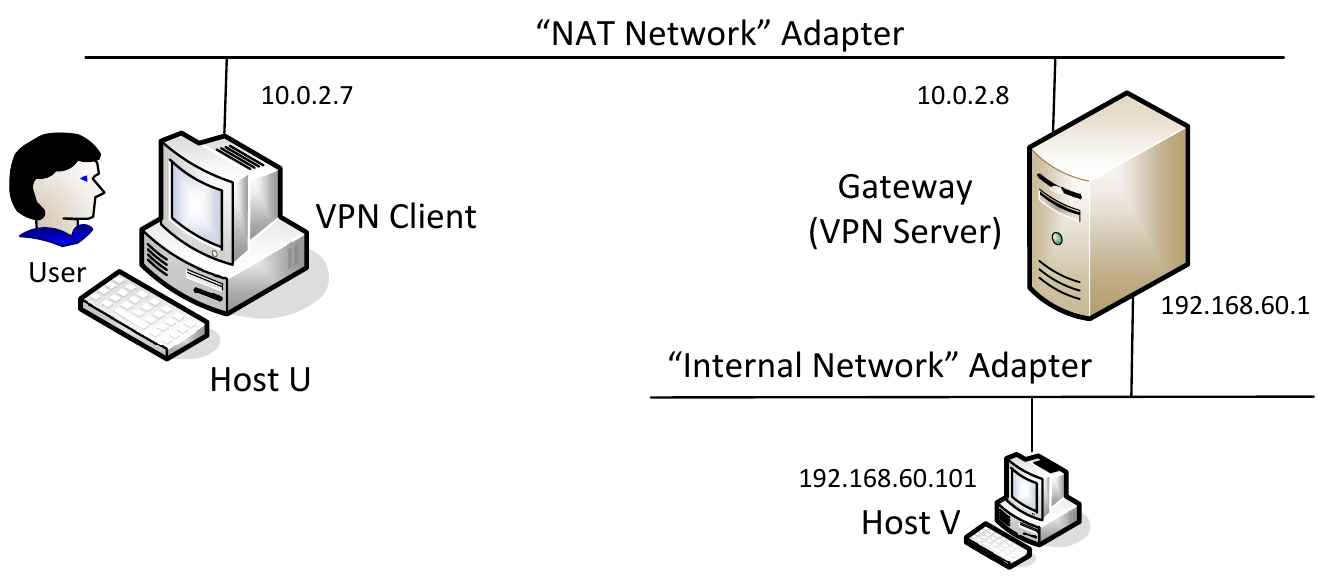
\includegraphics[scale=0.35]{t1_1.png}
    \end{center}{}
    \caption{VM setup for this lab}
    \label{fig:t1_1}
\end{figure}

Figure~\ref{fig:t1_1} shows the network graph of how the VM's should lay out. For redundancy, the IP address table is shown below:

\begin{center}
\begin{tabular}{ |c|c|c| } 
 \hline
 host & IP address(es) \\ 
 \hline
 client & 10.0.2.7  \\ 
 server & 10.0.2.8/192.168.60.1  \\ 
 target & 192.168.60.101 \\
 \hline
\end{tabular}
\end{center}

\subsubsection{Setting up NAT Network}
    The first step to setting up the environment in virtualbox is to set up a NAT Network.
    
    
    \begin{figure}[H]
        \begin{center}
            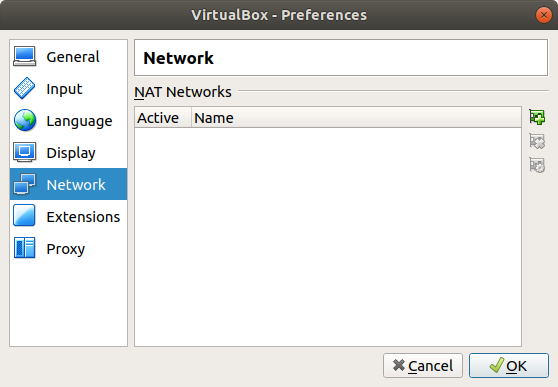
\includegraphics[scale=0.5]{NATNetwork_1.png}
        \end{center}{}
        \caption{VirtualBox Manager Preferences window}
        \label{fig:t1_2}
    \end{figure}
    
    Figure~\ref{fig:t1_2} shows the Virtualbox Manager Preferences window in which the Network tab is selected. Create a new NAT Network by clicking the green plus icon on the top right. 
    
    \begin{figure}[H]
        \begin{center}
            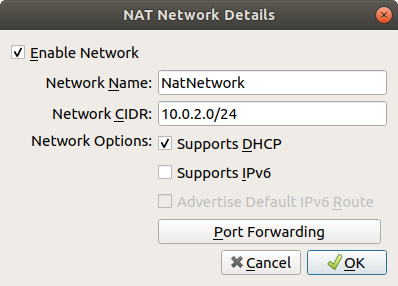
\includegraphics[scale=0.5]{NATNetwork_2.png}
        \end{center}{}
        \caption{Creating new NAT Network}
        \label{fig:t1_3}
    \end{figure}
    
    Figure~\ref{fig:t1_3} shows the window for creating a new NAT Network. Simply keep the defaults as they are and press OK.

\subsubsection{Setting up server settings}
    To set up the server settings through Virtualbox Manager, follow the following steps:
    \begin{enumerate}
        \item open up the settings of the \textbf{server} virtual machine
        \item click \textbf{Network} in the left column
        \item Open \textbf{Adapter 2} tab on the top
        \item create an internal network by changing \textbf{Attached to:} dropdown to \textbf{Internal Network}. Give the internal network a name. We used vpnnet.
    \end{enumerate}
    
    \begin{figure}[H]
        \begin{center}
            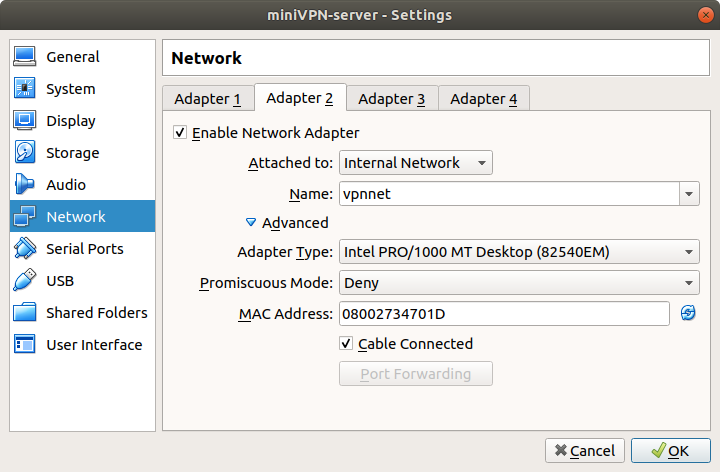
\includegraphics[scale=0.5]{networking_server.png}
        \end{center}{}
        \caption{Server Adapter 2 settings}
        \label{fig:networking_server}
    \end{figure}
    
    Figure~\ref{fig:networking_server} shows the Network settings for the internal network to attach to the target machine. Now we need to set up the public network for the client to access.
    
    \begin{enumerate}
        \item Open \textbf{Adapter 1} tab on the top
        \item Set Adapter 1 to \textbf{Nat Network}, and then choose the NAT Network we created earlier in Figure~\ref{fig:t1_3}
        
    \end{enumerate}
    \begin{figure}[H]
        \begin{center}
            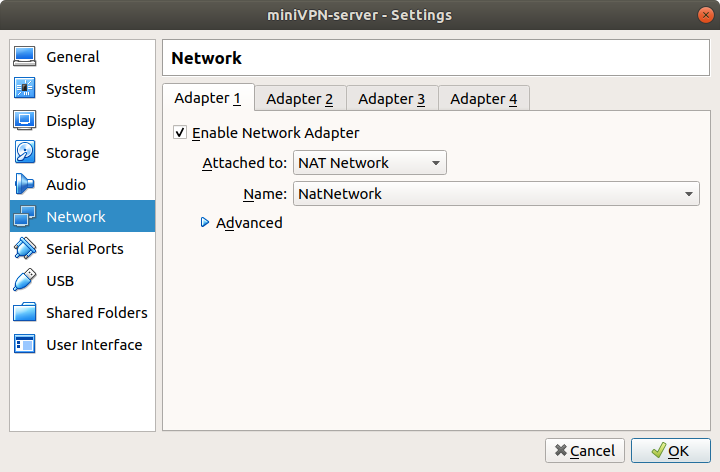
\includegraphics[scale=0.5]{networking_server2.png}
        \end{center}{}
        \caption{Server Adapter 1 settings}
        \label{fig:networking_server_2}
    \end{figure}
    
    Figure~\ref{fig:networking_server_2} shows the network settings for The Adapter 1 for the server. This is the adapter that the client will be accessing as mentioned previously. 

\subsubsection{Setting up target settings}
    \begin{enumerate}
        \item open up the settings of the \textbf{target} virtual machine
        \item click \textbf{Network} in the left column
        \item create an internal network by changing \textbf{Attached to:} dropdown to \textbf{Internal Network}. Give the internal network a name. We used vpnnet.
    \end{enumerate}
    
    \begin{figure}[H]
        \begin{center}
            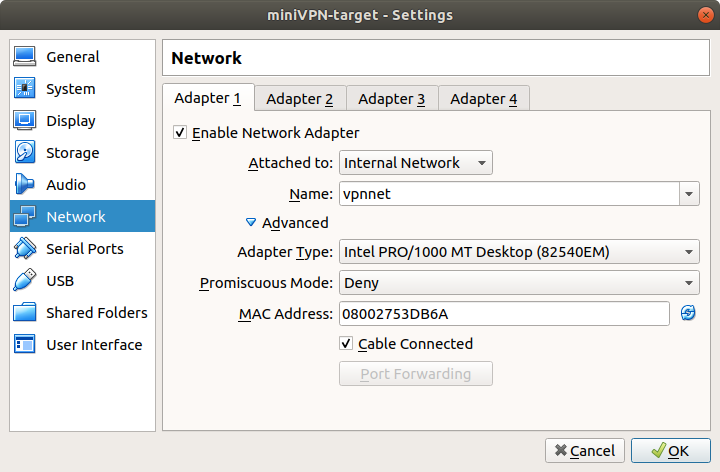
\includegraphics[scale=0.5]{networking_target.png}
        \end{center}{}
        \caption{Server Adapter 2 settings}
        \label{fig:networking_target}
    \end{figure}

\subsubsection{Setting up client settings}
    \begin{enumerate}
        \item open up the settings of the \textbf{client} virtual machine
        \item click \textbf{Network} in the left column
        \item Set Adapter 1 to \textbf{Nat Network}, and then choose the NAT Network we created earlier in Figure~\ref{fig:t1_3}
    \end{enumerate}
    
    \begin{figure}[H]
        \begin{center}
            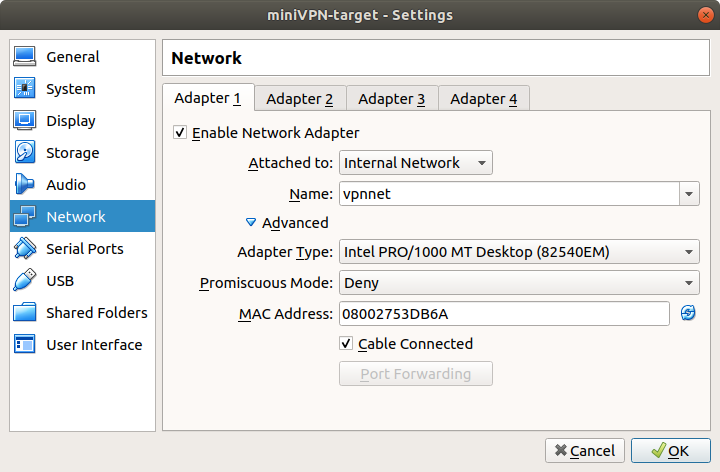
\includegraphics[scale=0.5]{networking_target.png}
        \end{center}{}
        \caption{Server Adapter 2 settings}
        \label{fig:networking_target}
    \end{figure}

\subsubsection{Setting up networking inside the Virtual Machines}

\paragraph{Server}

    Log into your \textbf{server} machine and on the top right click the icon to open the dropdown menu. 
    \begin{figure}[H]
        \begin{center}
            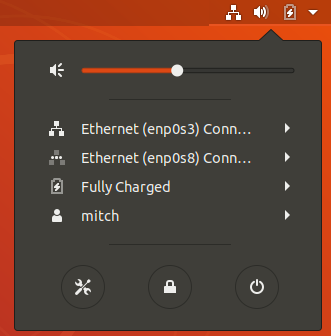
\includegraphics[scale=0.5]{setting_up_server_1.png}
        \end{center}{}
        \caption{Ubuntu 18.04 top right dropdown menu}
        \label{fig:setting_up_server_1}
    \end{figure}
    
    Figure~\ref{fig:setting_up_server_1} shows the drop down menu for Ubuntu 18.04 and two adapters can be seen. enp0s3 is the NAT Network Adapter, whereas enp0s8 is the internal network adapter. Edit the internal network adapter.
    
    \begin{figure}[H]
        \begin{center}
            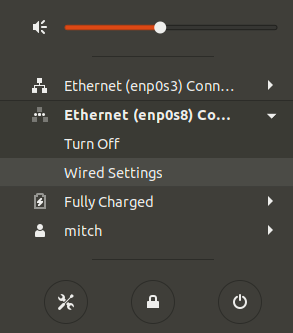
\includegraphics[scale=0.5]{setting_up_server_2.png}
        \end{center}{}
        \caption{Editing Network Adapter Through Menu}
        \label{fig:setting_up_server_2}
    \end{figure}

    Figure~\ref{fig:setting_up_server_2} shows what happens when you expand the network adapter. Simply click Wired Settings now.
    
    \begin{figure}[H]
        \begin{center}
            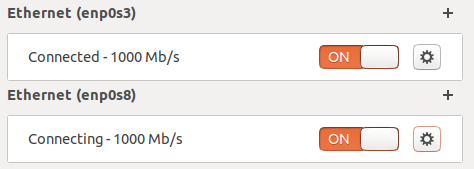
\includegraphics[scale=0.5]{setting_up_server_3.png}
        \end{center}{}
        \caption{Editing Network Adapter Through Menu}
        \label{fig:setting_up_server_3}
    \end{figure}

    You will see Figure~\ref{fig:setting_up_server_3} after clicking Wired Settings, and again, two adapters will be noticed. Click the cog next to the internal network adapter.

    Follow the following guide:
    \begin{enumerate}
        \item Click the \textbf{IPv4} tab
        \item check off \textbf{Manual} in the IPv4 Method section
        \item write the following network settings as shown in Figure~\ref{fig:setting_up_server_4}
    \end{enumerate}

    \begin{figure}[H]
        \begin{center}
            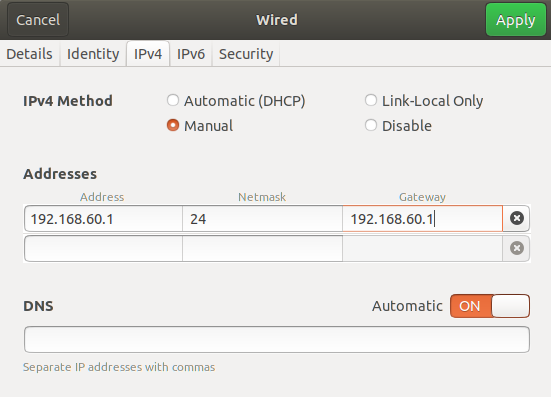
\includegraphics[scale=0.5]{setting_up_server_4.png}
        \end{center}{}
        \caption{Editing Network Adapter Through Menu}
        \label{fig:setting_up_server_4}
    \end{figure}

    Figure~\ref{fig:setting_up_server_4} Shows the final screen for editing the network adapter. Press Apply and then the internal network for the server is set. Now we need to set a static IP address for the public network.
    
    \begin{enumerate}
        \item open a terminal with \textbf{ctrl + alt + t}
        \item edit etc/network/interfaces and add the following
    \end{enumerate}
    
    \begin{verbatim}
    auto enp0s3
    iface enp0s3 inet static
        address 10.0.2.8
        netmask 255.255.255.0
        gateway 10.0.2.1
        dns-nameservers 8.8.8.8 8.8.4.4
    \end{verbatim}
    After adding the static network settings, either restart the system or execute the following:
    \begin{verbatim}
    $ sudo ip a flush enp0s3
    $ sudo systemctl restart networking.service
    \end{verbatim}
    
\paragraph{Target}
    
Similar to the Server, set up the networking as such:
    \begin{figure}[H]
        \begin{center}
            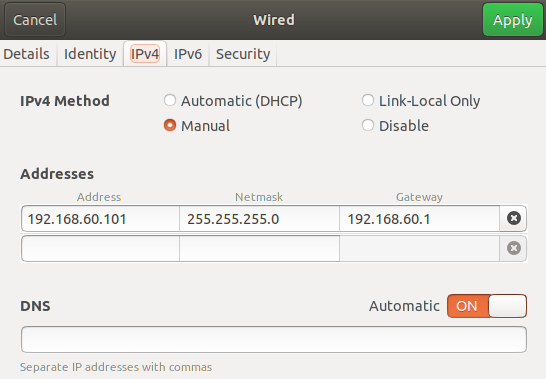
\includegraphics[scale=0.5]{setting_up_target_1.png}
        \end{center}{}
        \caption{target network settings}
        \label{fig:setting_up_target_1}
    \end{figure}


\paragraph{Client}

    Similar to the server, set up the static IP for the NAT Network.

    \begin{enumerate}
        \item open a terminal with \textbf{ctrl + alt + t}
        \item edit /etc/network/interfaces and add the following
    \end{enumerate}
    
    \begin{verbatim}
    auto enp0s3
    iface enp0s3 inet static
        address 10.0.2.7
        netmask 255.255.255.0
        gateway 10.0.2.1
        dns-nameservers 8.8.8.8 8.8.4.4
    \end{verbatim}
    
    An example file is shown below:
    
    \begin{figure}[H]
        \begin{center}
            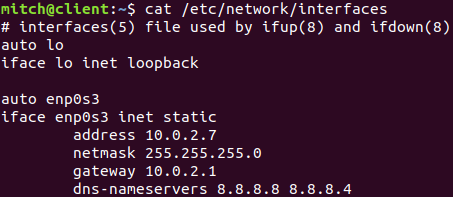
\includegraphics[scale=0.5]{setting_up_client_2.png}
        \end{center}{}
        \caption{example /etc/network/interfaces file}
        \label{fig:setting_up_client_2}
    \end{figure}
    
    
    After adding the static network settings, either restart the system or execute the following:
    \begin{verbatim}
    $ sudo ip a flush enp0s3
    $ sudo systemctl restart networking.service
    \end{verbatim}


\clearpage
\subsection{Task 2: Creating a VPN Tunnel using TUN/TAP}
    Creating a tunnel in this lab setup requires following all of the steps in Task 1. 

    The following section uses code provided by Syracuse University. The code samples can be found here - \url{https://seedsecuritylabs.org/Labs_16.04/Networking/VPN/} And contains source code for the TUN/TAP tunnels.

\subsubsection{setting up Server routing and interfaces}
    On the server, we need to start the vpn server provided by Syracuse University. Run the following command:
    
    \begin{verbatim}
        $ sudo ./vpnserver
    \end{verbatim}
    
    the vpnserver application is a blocking application, so we need to open a new terminal and set up the TUN and permit packet forwarding with:
    
    \begin{verbatim}
        $ sudo ifconfig tun0 192.168.53.1/24 up
        $ sudo sysctl net.ipv4.ip_forward=1
    \end{verbatim}
    
    \begin{figure}[H]
        \begin{center}
            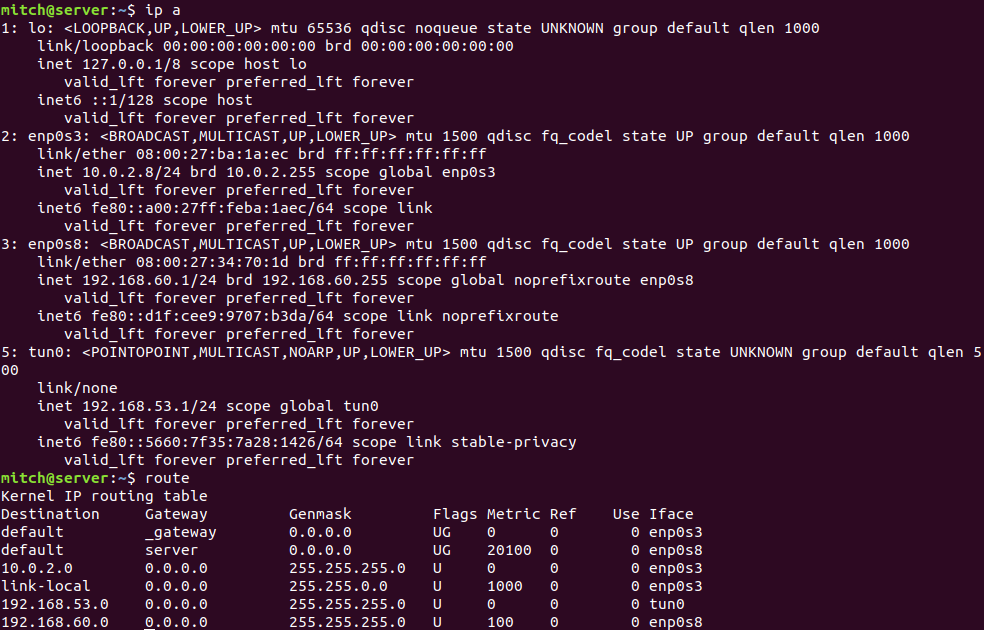
\includegraphics[scale=0.45]{t2_server_routing.png}
        \end{center}{}
        \caption{Task 2 Server Routing and Interfaces}
        \label{fig:t2_server_routing}
    \end{figure}

    Figure~\ref{fig:t2_server_routing} shows the routing and interfaces that the server should show. It can be seen that all 192.168.53.X traffic gets routed to the tun0 interface, whereas all the 192.168.60.X traffic is routed to the enp0s8 interface which is the internal network interface that our target machine is connected to. It can also be seen that tun0 is working and tied to the address 192.168.53.1.

\subsubsection{setting up Client routing and interfaces}
    On the Client, a slight modification to the source code is made. Figure~\ref{fig:t2_modify_vpnclient} shows the change to vpnclient.c which is just a change in one line.
    
    \begin{figure}[H]
        \begin{center}
            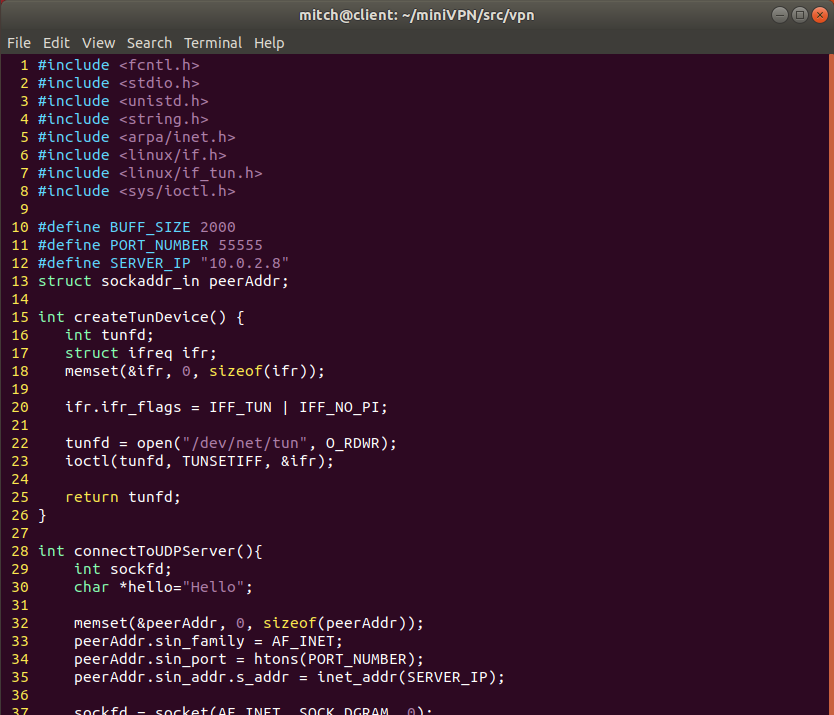
\includegraphics[scale=0.45]{t2_mody_vpnclient.png}
        \end{center}{}
        \caption{Task 2 Modifying vpnclient}
        \label{fig:t2_modify_vpnclient}
    \end{figure}

    In Figure~\ref{fig:t2_modify_vpnclient} it can be seen that line 12 is modified compared to the original source code. The SERVER$\_$IP is hardcoded into the file which we found necessary. When running the progrma while passing through the server IP, the tunnel did not pass through any packets properly.

    After the change in soure code, start the server and create the TUN interface as such:
    \begin{verbatim}
        $ sudo ./vpnclient
    \end{verbatim}
    Just like the server, vpnclient is a blocking application. Therefore, open up a new terminal and set up the interafces as such:
    \begin{verbatim}
        $ sudo ifconfig tun0 192.168.53.5/24 up
        $ sudo route add -net 192.168.60.0/24 tun0
    \end{verbatim}

    \begin{figure}[H]
        \begin{center}
            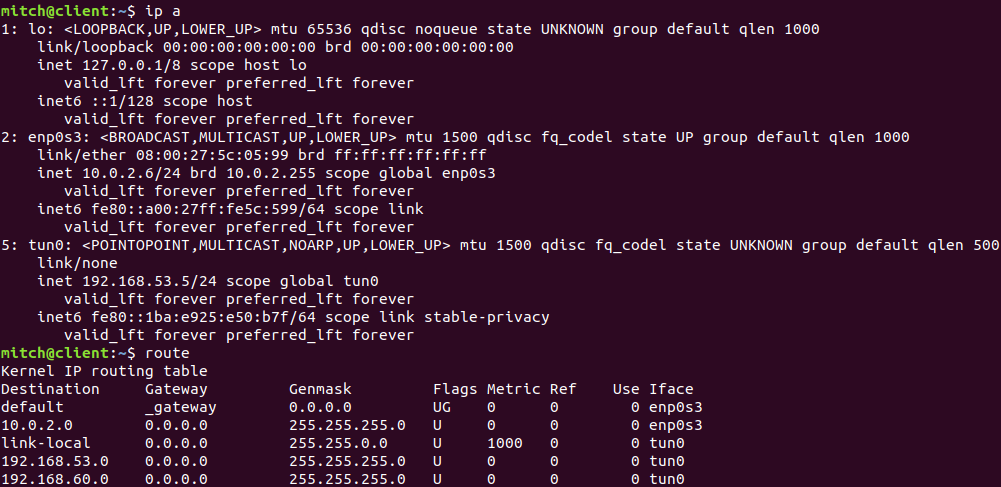
\includegraphics[scale=0.45]{t2_client_routing.png}
        \end{center}{}
        \caption{Task 2 Client Machine Routing and Interfaces}
        \label{fig:t2_client_routing}
    \end{figure}
    
    Figure~\ref{fig:t2_client_routing} shows the routing and network interfaces that the client machine should show. It can be seen all traffic going to 192.168.60.X and 192.168.53.X is being routed to the tun0 interface. It can also be seen that the tun0 interface is linked to the address 192.168.53.5.
    
    
\subsubsection{setting up Target routing and interfaces}
    Setting up the target machine is very simple, it is just adding one route to the routing table. And that route is sending 10.0.2.X traffic back to the server.
    \begin{verbatim}
        $ sudo route add -net 10.0.2.0/24 enp0s3    
    \end{verbatim}

    \begin{figure}[H]
        \begin{center}
            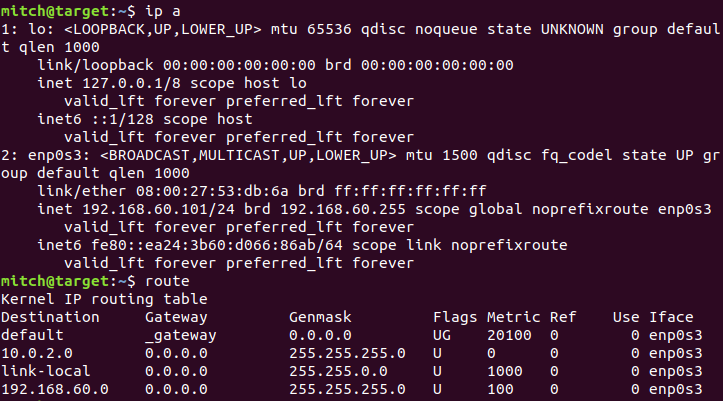
\includegraphics[scale=0.45]{t2_target_routing.png}
        \end{center}{}
        \caption{Task 2 Target Machine Routing and Interfaces}
        \label{fig:t2_target_routing}
    \end{figure}
    
    Figure~\ref{fig:t2_target_routing} shows the routing and network interfaces table. The only addition is adding the 10.0.2.X packets being routed to enp0s3.

\subsubsection{Ping Test}
    We wanted to make sure the ICMP packets from the ping utility command were actually reaching the target. Therefore, we ran the following command on the target:
    \begin{verbatim}
        $ sudo tcpdump ip proto \\icmp
    \end{verbatim}
    The previous command monitors all incoming TCP packets and prints out the icmp packets.

    \begin{figure}[H]
        \begin{center}
            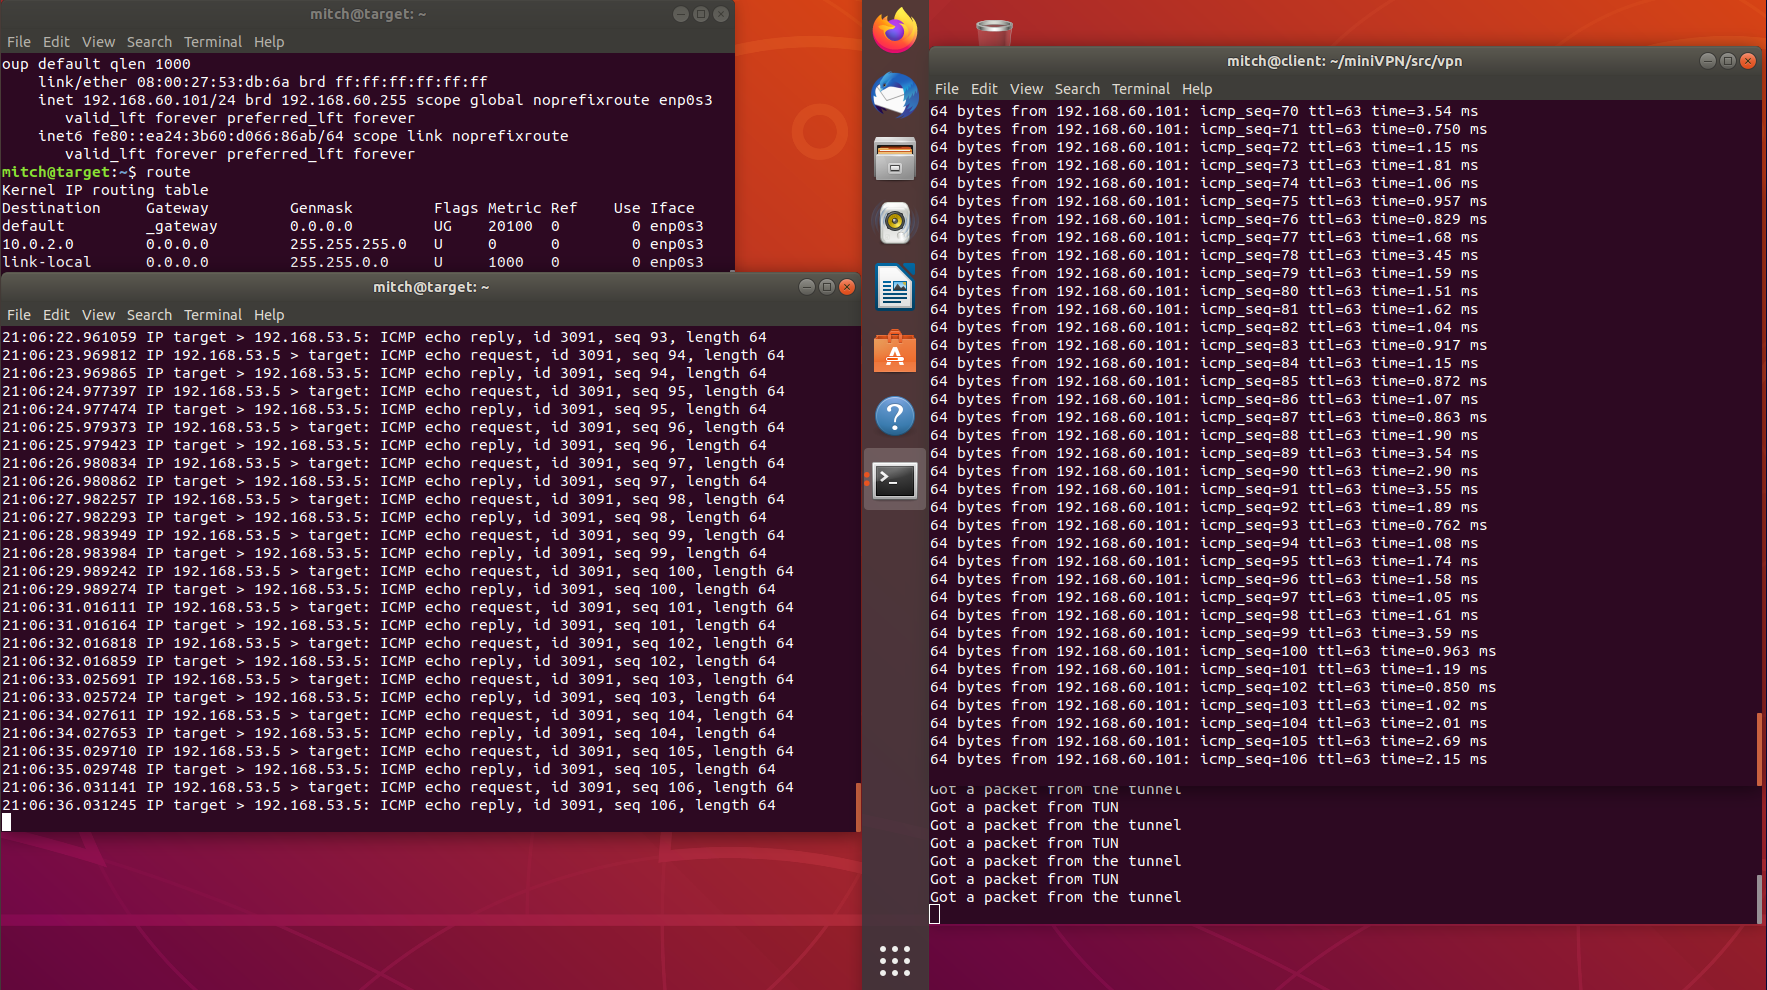
\includegraphics[scale=0.25]{t2_successful_ping.png}
        \end{center}{}
        \caption{Task 2 Client pinging Target}
        \label{fig:t2_successful_ping}
    \end{figure}
    
    Figure~\ref{fig:t2_successful_ping} shows the client machine successfully pinging the target machine. Doing the test is as simple as running the following command on the Client machine:
    
    \begin{verbatim}
        $ ping 192.168.60.101
    \end{verbatim}

    which is successful!
\subsubsection{Tunnel-Breaking Test}
    Due to the fact that our machines are running base Ubuntu 18.04, the telnetd package was needed to be downloaded onto the target machine. After that, we can telnet from the client machine to the target machine with:
    \begin{verbatim}
        $ telnet 192.168.60.101
    \end{verbatim}

    And then make sure that the tunnel is working properly. To do this, we did something simple such as 'touch test1' and verify that the file is created on the target. From there, we break the tunnel with the following command:
    \begin{verbatim}
        sudo ifconfig tun0 down
    \end{verbatim}
    
    Figure~\ref{fig:t2_breaking_tunnel} shows the results of setting the tun0 interface down

    \begin{figure}[H]
        \begin{center}
            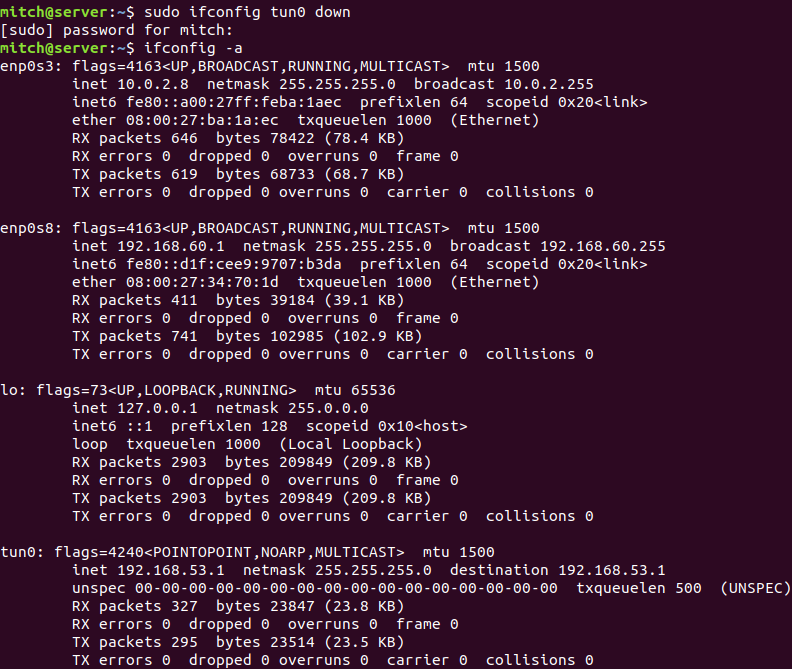
\includegraphics[scale=0.5]{t2_breaking_tunnel.png}
        \end{center}{}
        \caption{Task 2 Breaking VPN Tunnel}
        \label{fig:t2_breaking_tunnel}
    \end{figure}

    Figure~\ref{fig:t2_telnet_tunnel_break} shows the complete flow from initial connection to breaking to reconnection. 

    \begin{figure}[H]
        \begin{center}
            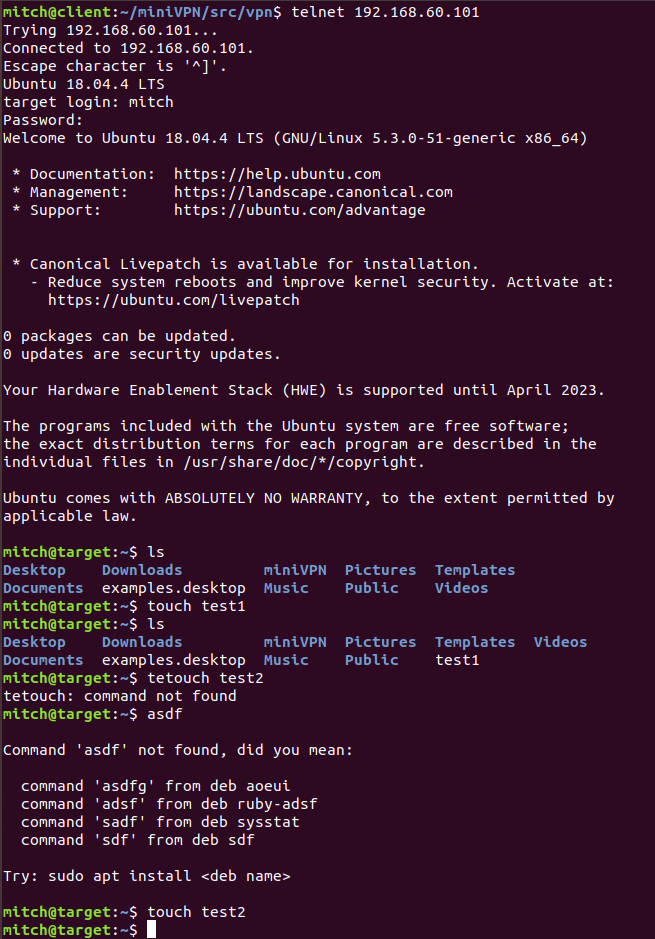
\includegraphics[scale=0.5]{t2_telnet_tunnel_break.png}
        \end{center}{}
        \caption{Task 2 Telnet Tunnel Break Test}
        \label{fig:t2_telnet_tunnel_break}
    \end{figure}

    What was noticed in the lab is that once the tunnel was broken, all keystrokes were frozen in the machine. After reconnecting to the machine, the commands suddenly came back and went through! The commands written during the broken tunnel were 'tetouch test' and 'asdf'. These commands did not show up when written while the tunnel was down, but came back when the tunnel was re-connected. The file test2 was shown on the target machine!

\subsection{Task 3: Set up Routing on Client and Server VMs}
\subsection{Task 4: Authenticating the VPN Server}
\textbf{Three Important Steps in Server Authentication:}
\begin{enumerate}
\item Verifying that the Server Certificate is Valid
\item Verifying that the Server is the Owner of the Certificate
\item Verifying that the Server is the Intended Server
\end{enumerate}
\textbf{Demonstrate two different cases regarding the third verification:}
\begin{enumerate}
\item  Successful Server Authentication where the server is the Intended Server
\item Failed Server Authentication where the server is not the Intended Server \\
\end{enumerate}
\textbf{Verifying that the Serve Certificate is Valid}
\item The certificate contains the server's public key, identity information, expiration date, CA's signature, and more relevant information; the most important information is the expiration date and signature. We know that the signature is valid because it will have the CA's public-key certificate, once the CA certificate is on the list, it can be directly verified. \\

\textbf{Verifying that the Server is the Owner of the Certificate}

\subsection{Task 5: Authenticating the VPN Client}
\subsection{Task 6: Supporting Multiple Clients}



\section{Conclusions}
VPN enables us to build a virtual private network over a public network, i.e. internet, such that connections with different users is protected regardless if the traffic goes through unprotected public networks.As shown in this lab, TSL/SSL provides privacy and data integrity between two or more communicating computer applications, i.e. client and sever. The connection is private because it uses symmetric cryptography to generate a shared secret key, which avoids the key distribution problem that other protocols encounter. 

\section{Future work and open problems}
\subsection{Future Work}
TSL/SSL VPN arose to solve the inability to support every multiple users while maintaining privacy. This protocol provides secure remote access via a web portal and nerwork-level access via SSL-secured tunnel between the client and network, with its main benefits of security and privacy. TSL/SSL VPN impacts future work drastically due to the growth of remote workforce, keeping employees connected to the work/academic applications they need and specifically for IT to ensure only authorized user gain access. 
\subsection{Open Problems}
\begin{itemize}
\item Implementation of TSL/SSL VPN requires products that support the current version of TLS because it is stronger than the older versions SSL. 
\end{itemize}
\begin{itemize}
\item An TSL/SSL VPN can attempt to ensure there is no carryover of sensitive information from session to session on a shared computer by wiping information, however it is not guarantee.
\end{itemize}


\section{Reference(s)}
\item Wenliang, D. (2019). "Chapter 12: Overview of Transport Layer Security".
\item 

\end{document}
